\documentclass[12pt]{article}
\usepackage{amsmath}
\usepackage{latexsym}
\usepackage{amsfonts}
\usepackage[normalem]{ulem}
\usepackage{soul}
\usepackage{array}
\usepackage{amssymb}
\usepackage{extarrows}
\usepackage{graphicx}
\usepackage[backend=biber,
style=numeric,
sorting=none,
isbn=false,
doi=false,
url=false,
]{biblatex}\addbibresource{bibliography.bib}

\usepackage{subfig}
\usepackage{wrapfig}
\usepackage{txfonts}
\usepackage{wasysym}
\usepackage{enumitem}
\usepackage{adjustbox}
\usepackage{ragged2e}
\usepackage[svgnames,table]{xcolor}
\usepackage{tikz}
\usepackage{longtable}
\usepackage{changepage}
\usepackage{setspace}
\usepackage{hhline}
\usepackage{multicol}
\usepackage{tabto}
\usepackage{float}
\usepackage{multirow}
\usepackage{makecell}
\usepackage{fancyhdr}
\usepackage[toc,page]{appendix}
\usepackage[hidelinks]{hyperref}
\usetikzlibrary{shapes.symbols,shapes.geometric,shadows,arrows.meta}
\tikzset{>={Latex[width=1.5mm,length=2mm]}}
\usepackage{flowchart}\usepackage[paperheight=11.69in,paperwidth=8.27in]{geometry}
\usepackage[utf8]{inputenc}
\usepackage[T1]{fontenc}
\TabPositions{0.5in,1.0in,1.5in,2.0in,2.5in,3.0in,3.5in,4.0in,4.5in,5.0in,5.5in,6.0in,}

\urlstyle{same}


 %%%%%%%%%%%%  Set Depths for Sections  %%%%%%%%%%%%%%

% 1) Section
% 1.1) SubSection
% 1.1.1) SubSubSection
% 1.1.1.1) Paragraph
% 1.1.1.1.1) Subparagraph


\setcounter{tocdepth}{5}
\setcounter{secnumdepth}{5}


 %%%%%%%%%%%%  Set Depths for Nested Lists created by \begin{enumerate}  %%%%%%%%%%%%%%


\setlistdepth{9}
\renewlist{enumerate}{enumerate}{9}
		\setlist[enumerate,1]{label=\arabic*)}
		\setlist[enumerate,2]{label=\alph*)}
		\setlist[enumerate,3]{label=(\roman*)}
		\setlist[enumerate,4]{label=(\arabic*)}
		\setlist[enumerate,5]{label=(\Alph*)}
		\setlist[enumerate,6]{label=(\Roman*)}
		\setlist[enumerate,7]{label=\arabic*}
		\setlist[enumerate,8]{label=\alph*}
		\setlist[enumerate,9]{label=\roman*}

\renewlist{itemize}{itemize}{9}
		\setlist[itemize]{label=$\cdot$}
		\setlist[itemize,1]{label=\textbullet}
		\setlist[itemize,2]{label=$\circ$}
		\setlist[itemize,3]{label=$\ast$}
		\setlist[itemize,4]{label=$\dagger$}
		\setlist[itemize,5]{label=$\triangleright$}
		\setlist[itemize,6]{label=$\bigstar$}
		\setlist[itemize,7]{label=$\blacklozenge$}
		\setlist[itemize,8]{label=$\prime$}

\setlength{\topsep}{0pt}\setlength{\parskip}{8.04pt}
\setlength{\parindent}{0pt}

 %%%%%%%%%%%%  This sets linespacing (verticle gap between Lines) Default=1 %%%%%%%%%%%%%%


\renewcommand{\arraystretch}{1.3}


%%%%%%%%%%%%%%%%%%%% Document code starts here %%%%%%%%%%%%%%%%%%%%



\begin{document}


%%%%%%%%%%%%%%%%%%%% Figure/Image No: 1 starts here %%%%%%%%%%%%%%%%%%%%

\begin{figure}[H]
	\begin{Center}
		
\includegraphics[width=3.71in,height=1.44in]{./media/image1.png}
	\end{Center}
\end{figure}


%%%%%%%%%%%%%%%%%%%% Figure/Image No: 1 Ends here %%%%%%%%%%%%%%%%%%%%

\par



%%%%%%%%%%%%%%%%%%%% Figure/Image No: 2 starts here %%%%%%%%%%%%%%%%%%%%

\begin{figure}[H]
	\begin{Center}
		
\includegraphics[width=3.08in,height=3.08in]{./media/image2.jpeg}
	\end{Center}
\end{figure}


%%%%%%%%%%%%%%%%%%%% Figure/Image No: 2 Ends here %%%%%%%%%%%%%%%%%%%%

\par


\vspace{\baselineskip}
\begin{Center}
 {\fontsize{16pt}{19.2pt}\selectfont \textbf{\uline{Faculty of Mathematics and Information Science}}\par}
\end{Center}\par


\vspace{\baselineskip}
\begin{Center}
{\fontsize{16pt}{19.2pt}\selectfont \textbf{\textcolor[HTML]{1F4E79}{\uline{User Guide for Deterministic Actions with Cost}}}\par}
\end{Center}\par


\vspace{\baselineskip}

\vspace{\baselineskip}

\vspace{\baselineskip}
{\fontsize{14pt}{16.8pt}\selectfont Submitted by: \tab \par}\par

\begin{adjustwidth}{0.5in}{0.0in}
{\fontsize{14pt}{16.8pt}\selectfont Haran Dev Murugan\par}\par

\end{adjustwidth}

\begin{adjustwidth}{0.5in}{0.0in}
{\fontsize{14pt}{16.8pt}\selectfont Rahul Tomer\par}\par

\end{adjustwidth}

\begin{adjustwidth}{0.5in}{0.0in}
{\fontsize{14pt}{16.8pt}\selectfont Rishabh Jain\par}\par

\end{adjustwidth}

\begin{adjustwidth}{0.5in}{0.0in}
{\fontsize{14pt}{16.8pt}\selectfont Kuldeep Shankar\par}\par

\end{adjustwidth}

\begin{adjustwidth}{0.5in}{0.0in}
{\fontsize{14pt}{16.8pt}\selectfont Alaa Abboushi\par}\par

\end{adjustwidth}

\begin{adjustwidth}{0.5in}{0.0in}
{\fontsize{14pt}{16.8pt}\selectfont Bui Tuan Anh. \tabto{2.71in} \tab \par}\par

\end{adjustwidth}


\vspace{\baselineskip}

\vspace{\baselineskip}
\section{Approver:\  Dr Anna Radzikowska}

\vspace{\baselineskip}

\vspace{\baselineskip}

\vspace{\baselineskip}
\tab \tab \tab \tab \tab \tab \tab {\fontsize{14pt}{16.8pt}\selectfont \tab Date:\  26/06/20\par}\par


\vspace{\baselineskip}

\vspace{\baselineskip}

\vspace{\baselineskip}

\vspace{\baselineskip}

\vspace{\baselineskip}
\textbf{Introduction: }\par

\tab A dynamic system is designed for deterministic actions with cost. This document will help a user to understand the design and functionality of the system.\par

Following workflow is performed based on our Example 1 (Travel -Fuel – Reserve) from our drafted functional document. As system is dynamic hence other examples can be verified exactly same way as shown below.\par

Numerical Indices shown in images have been explained respectively followed by image.\par


\vspace{\baselineskip}
System has been designed in C$\#$  language.\par


\vspace{\baselineskip}

\vspace{\baselineskip}
\textbf{Home Screen:}\par

\tab 
\vspace{\baselineskip}

%%%%%%%%%%%%%%%%%%%% Figure/Image No: 3 starts here %%%%%%%%%%%%%%%%%%%%

\begin{figure}[H]
	\begin{Center}
		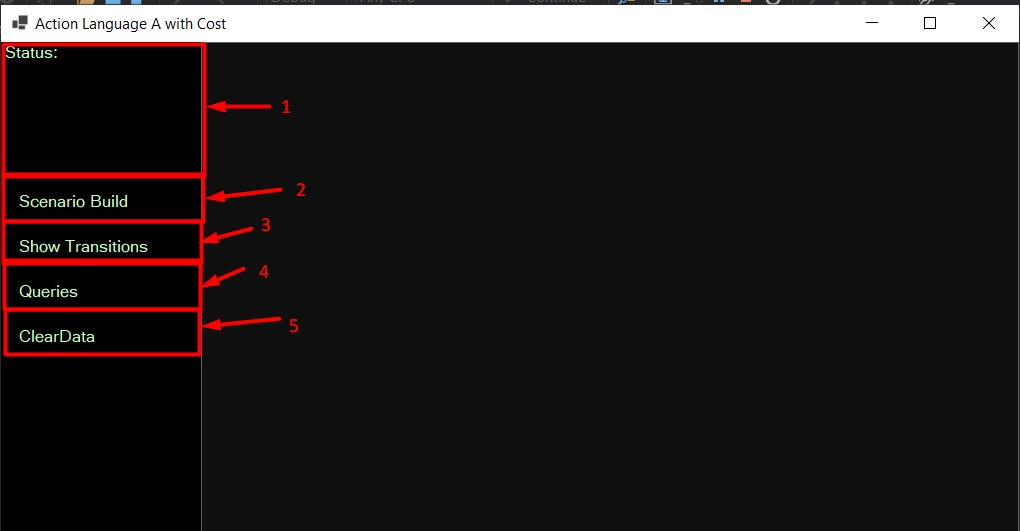
\includegraphics[width=6.27in,height=3.26in]{./media/image3.jpeg}
	\end{Center}
\end{figure}


%%%%%%%%%%%%%%%%%%%% Figure/Image No: 3 Ends here %%%%%%%%%%%%%%%%%%%%

\par


\vspace{\baselineskip}
\textbf{Legend:}\par


\vspace{\baselineskip}
\begin{enumerate}
	\item Status\par

\tab Displays the status of the project (If the fluents are submitted, if the actions are \tab added, If the states are added etc.)\par


\vspace{\baselineskip}
	\item Scenario Build\par

\tab This button is a drop-down menu button used for adding fluents and actions needed \tab for scenario building. (Refer the Next image)\par


\vspace{\baselineskip}
	\item Show Transitions\par

\tab This Button opens the show states form that lets us Set the initial state and then shows \tab the generated states and transitions of the system\par


\vspace{\baselineskip}
	\item Queries\par

\tab This Button opens the queries form window that lets us check a query against the \tab scenario that we have built.\par


\vspace{\baselineskip}
	\item Clear Data
\end{enumerate}\par

This Button clears all the data inputted by the user and reset the system.\par


\vspace{\baselineskip}

\vspace{\baselineskip}

\vspace{\baselineskip}
\textbf{Scenario Build:}\par


\vspace{\baselineskip}


%%%%%%%%%%%%%%%%%%%% Figure/Image No: 4 starts here %%%%%%%%%%%%%%%%%%%%

\begin{figure}[H]
	\begin{Center}
		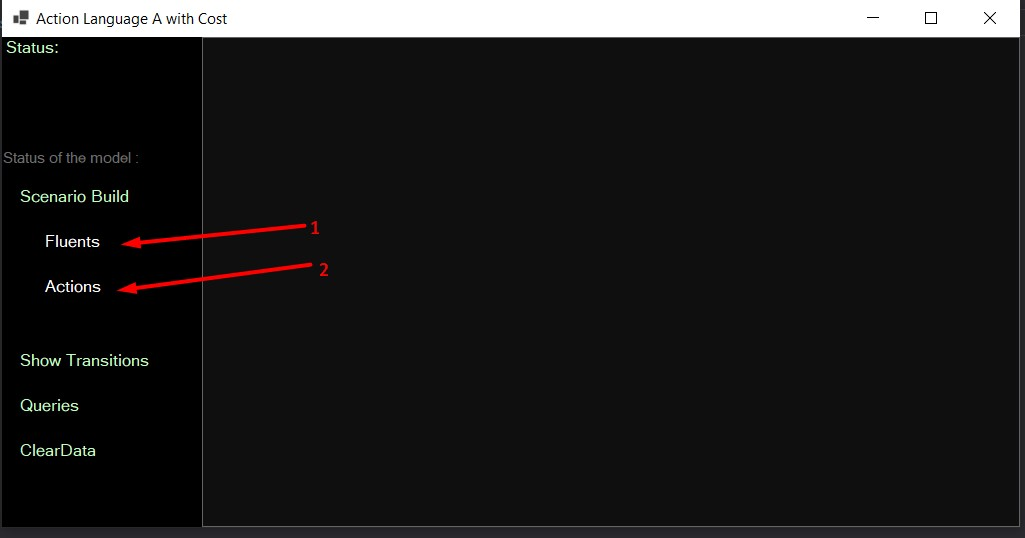
\includegraphics[width=6.26in,height=3.28in]{./media/image4.jpeg}
	\end{Center}
\end{figure}


%%%%%%%%%%%%%%%%%%%% Figure/Image No: 4 Ends here %%%%%%%%%%%%%%%%%%%%

\par


\vspace{\baselineskip}
\textbf{Legend:}\par


\vspace{\baselineskip}
\begin{enumerate}
	\item Fluents\tab \par

\tab This Displays the Add Fluents form window that lets us add fluents of the scenario\par


\vspace{\baselineskip}
	\item Actions
\end{enumerate}\par

\tab This button displays the Add Actions form window that lets us add actions and their \tab respective conditions to the scenario.\par


\vspace{\baselineskip}
\textbf{Fluents:}\par


\vspace{\baselineskip}


%%%%%%%%%%%%%%%%%%%% Figure/Image No: 5 starts here %%%%%%%%%%%%%%%%%%%%

\begin{figure}[H]
	\begin{Center}
		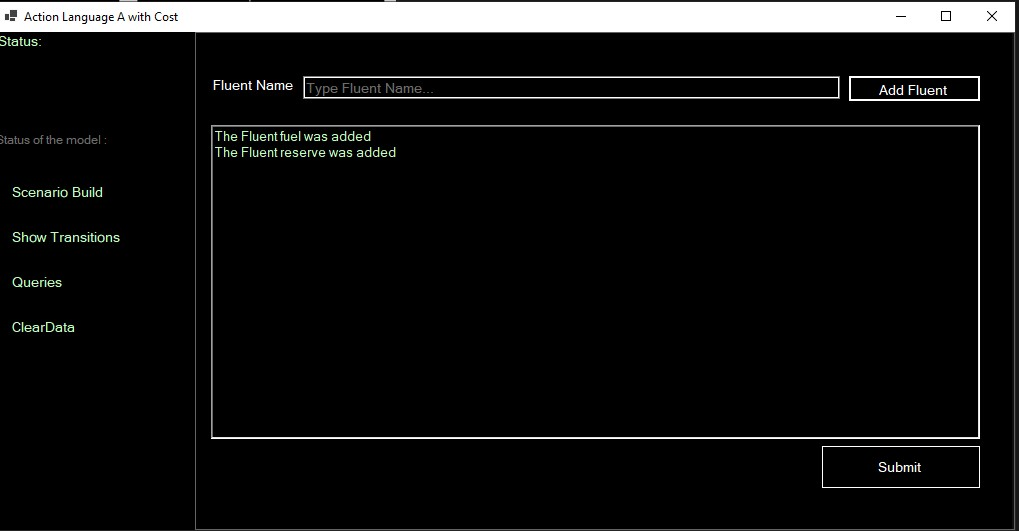
\includegraphics[width=6.27in,height=3.27in]{./media/image5.jpeg}
	\end{Center}
\end{figure}


%%%%%%%%%%%%%%%%%%%% Figure/Image No: 5 Ends here %%%%%%%%%%%%%%%%%%%%

\par


\vspace{\baselineskip}
How to Add Fluents\par


\vspace{\baselineskip}
\begin{enumerate}
	\item Type the name of the fluent name in the First Text box.\par

	\item Press add fluent\par

	\item Status of the addition will be displayed on the big text box\par

	\item Press submit button if all fluents are added. (Very important as it will change the status of fluents in the system)
\end{enumerate}\par


\vspace{\baselineskip}
\textbf{Actions:}\par


\vspace{\baselineskip}


%%%%%%%%%%%%%%%%%%%% Figure/Image No: 6 starts here %%%%%%%%%%%%%%%%%%%%

\begin{figure}[H]
	\begin{Center}
		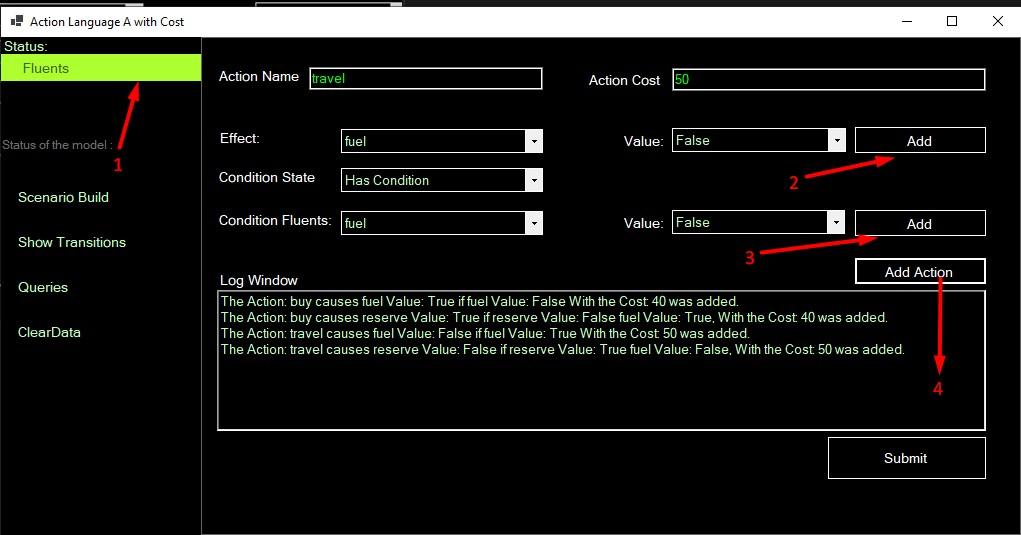
\includegraphics[width=6.26in,height=3.28in]{./media/image6.jpeg}
	\end{Center}
\end{figure}


%%%%%%%%%%%%%%%%%%%% Figure/Image No: 6 Ends here %%%%%%%%%%%%%%%%%%%%

\par


\vspace{\baselineskip}

\vspace{\baselineskip}

\vspace{\baselineskip}

\vspace{\baselineskip}
\textbf{Legend:}\par


\vspace{\baselineskip}
\begin{enumerate}
	\item The Status of adding fluents will turn green after you submit the fluents in the fluents form. If its red this Form will not be displayed because it is important for us to have fluents before adding actions.\par

	\item Add Effect Fluent Button.\par

	\item Add Condition Fluent Button.\par

	\item Add the Action.
\end{enumerate}\par


\vspace{\baselineskip}
How to Add Actions \par

\begin{enumerate}
	\item Type the action name and cost of the action.\par

	\item Select the effect fluent and its corresponding value in the Drop-down list and press button 2.\par

\begin{enumerate}
	\item Buy causes not fuel. For this we select fuel as effect and value as false and press button 2.\par

	\item Error message will be shown to user in case button 2 is pressed after adding one effect fluent already.\par


\end{enumerate}
	\item If\ the Action statement is $``$Buy Causes Fuel$"$ , we can keep the condition state as No Condition (Condition state drop down list). But if the action is  $``$ Buy causes fuel if.$"$ \ , then the condition state should be has condition which upon selecting will display the dropdown for condition fluents, their respective values and the add condition fluent button  (Button 3).\par

	\item Adding the Condition Fluents is as same as adding effect fluent only change is instead of button 2 its button 3.\par

	\item Add Action Button (Button 4) is pressed to add the action to the action list and display the log in the status textbox below.\par

	\item After adding all the actions press Submit Button (Very important!).
\end{enumerate}\par


\vspace{\baselineskip}
\textbf{States:}\par


\vspace{\baselineskip}


%%%%%%%%%%%%%%%%%%%% Figure/Image No: 7 starts here %%%%%%%%%%%%%%%%%%%%

\begin{figure}[H]
	\begin{Center}
		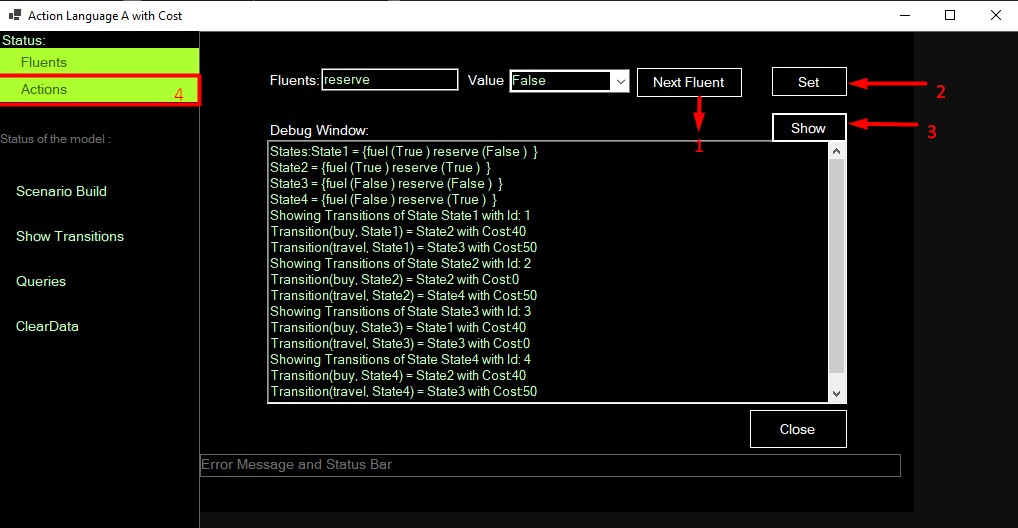
\includegraphics[width=6.26in,height=3.25in]{./media/image7.jpeg}
	\end{Center}
\end{figure}


%%%%%%%%%%%%%%%%%%%% Figure/Image No: 7 Ends here %%%%%%%%%%%%%%%%%%%%

\par

\textbf{Legend:}\par


\vspace{\baselineskip}
\begin{itemize}
	\item (4) The Status of adding Actions will turn green after you submit the Actions in the Actions form. If its red this Form will not be displayed because it is important for us to have Actions before setting initial state and generating transitions.
\end{itemize}\par

\begin{enumerate}
	\item This button is used to go to the next fluent after you have set the value of a respective fluent specified. if all fluents are set with respective values the status bar will prompt to set the initial state.\par

	\item Sets the initial state for the scenario with the values inputted by the user.\par

	\item Shows the generated states and transitions for the respective initial state, fluents and actions of the scenario in the Debug Window.\par

	\item The Button Close should be pressed after the transitions are shown and the results are verified because it will turn the states and transitions to be in green status, a prerequisite for the Queries Form.
\end{enumerate}\par


\vspace{\baselineskip}

\vspace{\baselineskip}
\textbf{Queries:}\par


\vspace{\baselineskip}


%%%%%%%%%%%%%%%%%%%% Figure/Image No: 8 starts here %%%%%%%%%%%%%%%%%%%%

\begin{figure}[H]
	\begin{Center}
		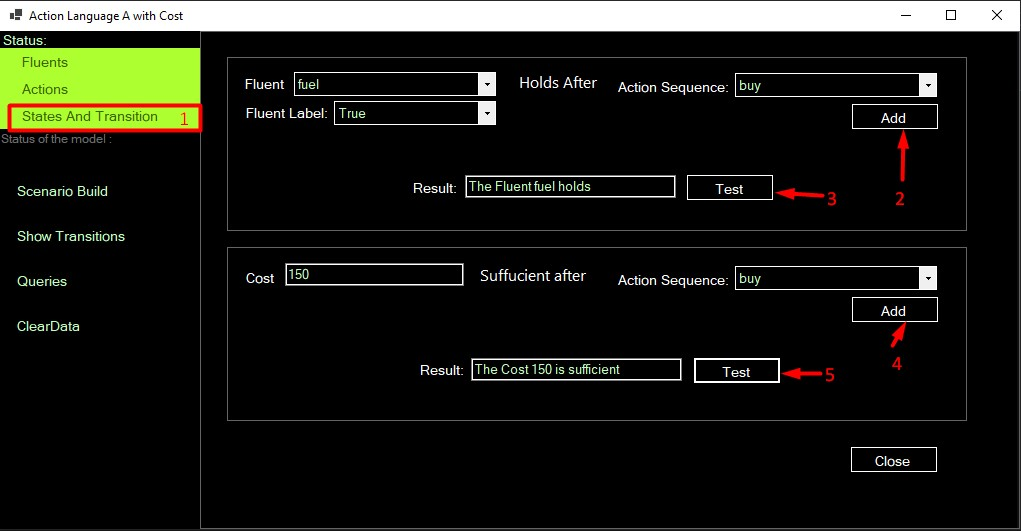
\includegraphics[width=6.26in,height=3.26in]{./media/image8.jpeg}
	\end{Center}
\end{figure}


%%%%%%%%%%%%%%%%%%%% Figure/Image No: 8 Ends here %%%%%%%%%%%%%%%%%%%%

\par


\vspace{\baselineskip}
\textbf{Legend:}\par


\vspace{\baselineskip}
\begin{enumerate}
	\item The Status of states and transitions will turn green after you close the show states form after setting the initial state and generating the various states and transitions. If its red this Form will not be displayed because it is important for us to have states and transitions generated before setting queries.\par

	\item The Add button adds the respective Action selected to the Action sequence.\par

	\item The button test is pressed after adding the Actions to the Action sequence and it will display if the fluent and value selected by the user holds or not in the Result Text Box.\par

	\item The Add button adds the respective Action selected to the Action sequence.\par

	\item The button test is pressed after adding the Actions to the Action sequence and it will display if the cost value submitted by the user is sufficient or not in the Result Text Box.
\end{enumerate}\par


\vspace{\baselineskip}
\textbf{Clear Data:}\par


\vspace{\baselineskip}
This Button clears all the data inputted by the user and reset the system.\par


\vspace{\baselineskip}

\vspace{\baselineskip}

\vspace{\baselineskip}

\vspace{\baselineskip}

\vspace{\baselineskip}

\vspace{\baselineskip}

\vspace{\baselineskip}

\vspace{\baselineskip}

\vspace{\baselineskip}

\vspace{\baselineskip}

\vspace{\baselineskip}

\vspace{\baselineskip}

\vspace{\baselineskip}

\vspace{\baselineskip}

\vspace{\baselineskip}

\vspace{\baselineskip}

\vspace{\baselineskip}

\vspace{\baselineskip}

\vspace{\baselineskip}

\vspace{\baselineskip}

\printbibliography
\end{document}